% !TeX program = xelatex
% !TeX encoding = UTF-8
\documentclass[a4paper, 11pt, answers]{exam}

\usepackage[brazil]{babel}
\let\latinencoding\relax
\usepackage[T1]{fontenc}

\usepackage[no-math]{fontspec}
\usepackage{newpxtext, newpxmath}
\usepackage[a4paper, margin=2cm]{geometry}

\usepackage{siunitx}
\usepackage{fancyvrb}
\usepackage{graphicx}
\usepackage{caption}
\usepackage{siunitx}
\usepackage{microtype}
\PassOptionsToPackage{hyphens}{url}
\usepackage[colorlinks,breaklinks=true,urlcolor=blue,linkcolor=black]{hyperref}
\def\UrlBreaks{\do\/\do-}
%\usepackage[hyphenbreaks]{breakurl}

\input{definition.tex}

\title{\titulo}
\author{\nomeAutorUm e \nomeAutorDois}
\date{\today}

\footer{}{}{\thepage}

\sisetup{
  binary-units = true
}

\renewcommand{\solutiontitle}{}

\fvset{
  gobble=8,
  frame = single
}

\graphicspath{{img/}}

\newcommand{\printtitle}{
  \begin{center}
    {\Large \scshape \titulo}\\[1em]
    {\nomeAutorUm, \raAutorUm}\\
    {\nomeAutorDois, \raAutorDois}\\[1em]
    Professor: Dr\@. \nomeProfessor, \centroProfessor\\
    {\itshape \campusFaculdade}
  \end{center}
}

\begin{document}
  \printtitle

  \begin{questions}
    \question
    Aplicação UDP.

    \begin{parts}
      \part
      Execute a aplicação socket UDP cliente/servidor em Java. Envie uma
      mensagem de um cliente para o servidor (em outra máquina do laboratório),
      capturando os pacotes enviados com o Wireshark. Selecione um pacote UDP.

      \begin{subparts}
        \subpart
        Quantos e quais são os campos do cabeçalho UDP?

        \begin{solution}
          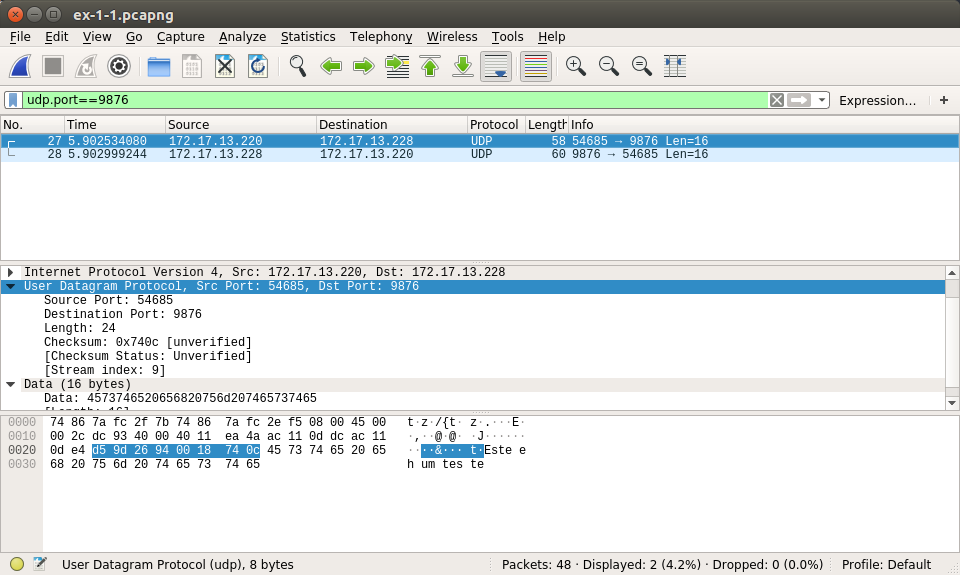
\includegraphics[width=\linewidth]{ex-1-1-1.png}
          \captionof{figure}{Campos presentes no cabeçalho UDP.}
          \vspace{1em}

          O cabeçalho possui quatro campos: a porta de origem, porta de 
          destino, tamanho e \emph{checksum}, como pode-se observar
          na figura acima.
        \end{solution}

        \subpart
        O valor no campo \emph{length} (comprimento) é o comprimento do que?
        Do cabeçalho, dados ou do pacote UDP inteiro?

        \begin{solution}
          É o comprimento do cabeçalho do UDP somado a carga útil, totalizando,
          portanto, o comprimento do pacote UDP inteiro.
        \end{solution}

        \subpart
        Qual é o maior número possível de porta de origem no UDP? E de
        destino? Justifique.

        \begin{solution}
          As portas utilizam \SI{2}{bytes}, sendo inteiros não negativos.
          O maior número possível de porta de origem e de destino é, portanto,
          $65535$.
        \end{solution}

        \pagebreak
        \subpart
        Qual é o número de protocolo para o UDP? (Para responder, você
        precisa verificar no cabeçalho IP).

        \begin{solution}
          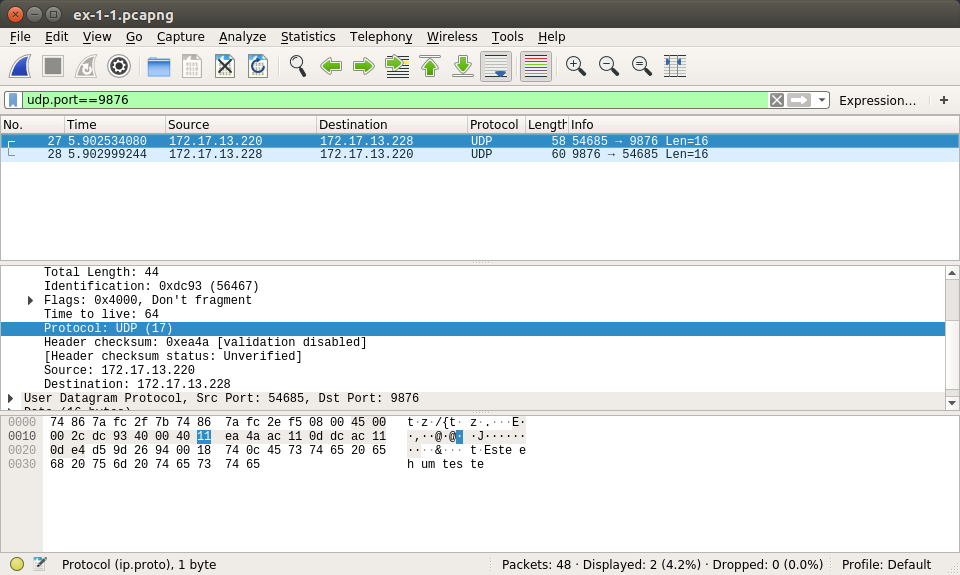
\includegraphics[width=\linewidth]{ex-1-1-4.png}
          \captionof{figure}{Número de protocolo utilizado pelo UDP.}
          \vspace{1em}

          O UDP utiliza como número de protocolo o 17, como pode-se observar
          no cabeçalho IP na figura acima.
        \end{solution}
      \end{subparts}

      \part
      Examine um par de pacotes UDP em que o primeiro pacote é enviado
      pelo cliente e o segundo pacote é a resposta do servidor a este pacote.
      Descreva a relação entre os números de portas nos dois pacotes.

      \begin{solution}
        A porta de destino é a qual o servidor está executando o programa
        quando o cliente manda a mensagem. A partir do momento que o servidor
        responde, a porta de origem passa a ser a de destino original,
        havendo uma inversão. Desta forma, identifica-se de forma única
        uma comunicação entre dois \emph{hosts}.
      \end{solution}
    \end{parts}

    \question
    Aplicação TCP.

    \begin{parts}
      \part
      Execute a aplicação socket TCP cliente/servidor em Java. Envie uma
      mensagem de um cliente para o servidor (em outra máquina do laboratório),
      capturando os pacotes enviados com o Wireshark.

      \begin{subparts}
        \pagebreak
        \subpart
        Quantos e quais são os campos do cabeçalho TCP?

        \begin{solution}
          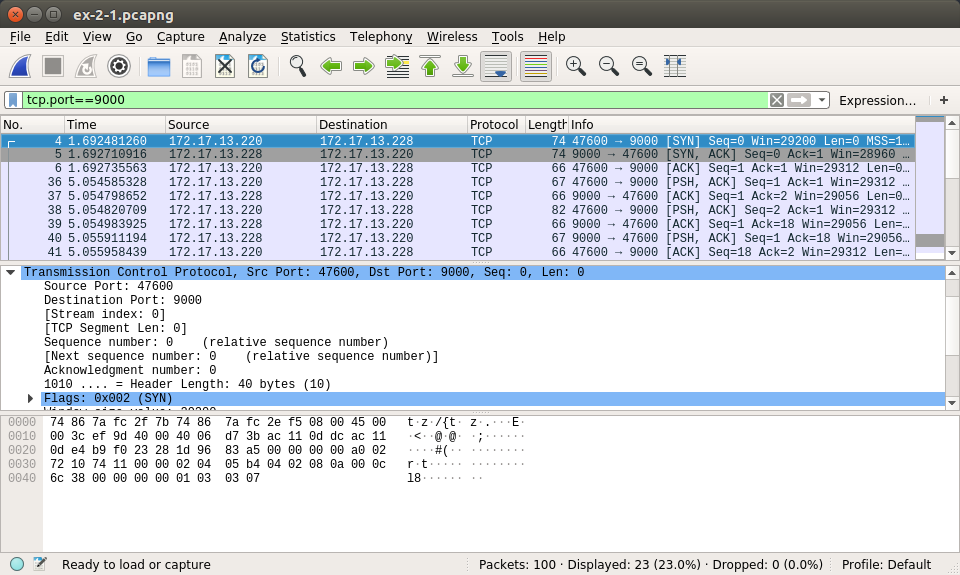
\includegraphics[width=\linewidth]{ex-2-1-1.png}
          \captionof{figure}{Alguns dos campos do cabeçalho TCP.}
          \vspace{1em}

          O cabeçalho TCP possui 9 campos, sendo estes: porta de origem
          e de destino, número de sequência e de \emph{acknowledgment},
          as \emph{flags}, valor de janela, \emph{checksum} e ponteiro
          de urgente, além das opções e tamanho de cabeçalho.
        \end{solution}

        \subpart
        Qual é o endereço IP e porta TCP usado pelo cliente? E pelo servidor?

        \begin{solution}
          O cliente atua no endereço IP \verb|172.17.13.220| na porta 
          \verb|9000| e o servidor responde pelo IP \verb|172.17.13.228|
          na porta \verb|47600| do cliente.
        \end{solution}

        \subpart
        Execute novamente o cliente. Verifique a porta e IP do cliente.

        \begin{solution}
          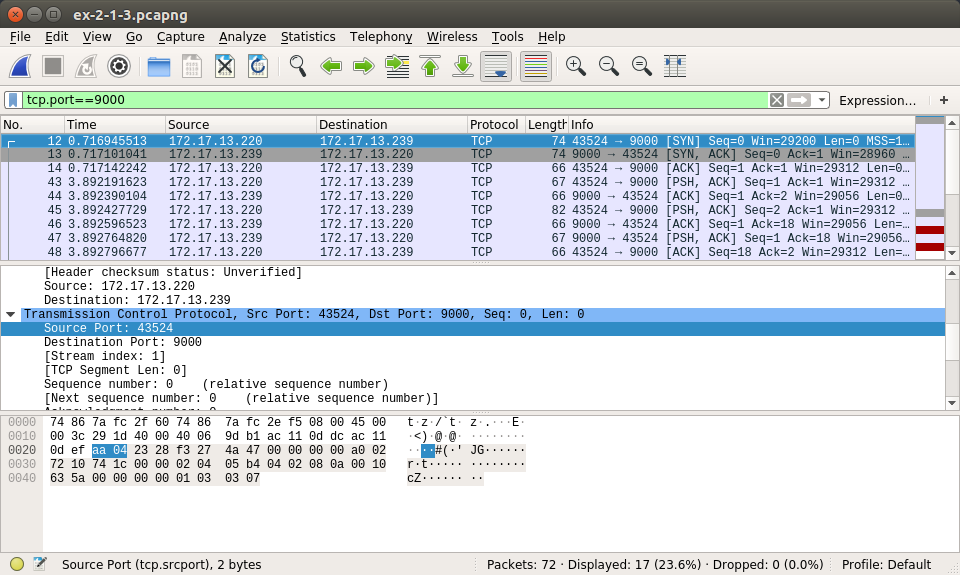
\includegraphics[width=\linewidth]{ex-2-1-3.png}
          \captionof{figure}{Nova porta utilizada pelo cliente.}
          \vspace{1em}

          Mudou-se a porta de destino do cliente, para possibilitar
          com que haja a identificação correta visto que é um outro processo.
        \end{solution}

        \subpart
        Qual o número de sequência do segmento TCP SYN usado para iniciar a
        conexão TCP entre cliente e servidor? Qual é o número do segmento
        SYNACK enviado pelo servidor em resposta ao SYN enviado pelo cliente?
        Qual o valor do campo de reconhecimento do cabeçalho TCP para o 
        segmento SYNACK? Como o servidor determinou este valor? Explique
        como funciona todo este processo de estabelecimento de conexão TCP.

        \begin{solution}
          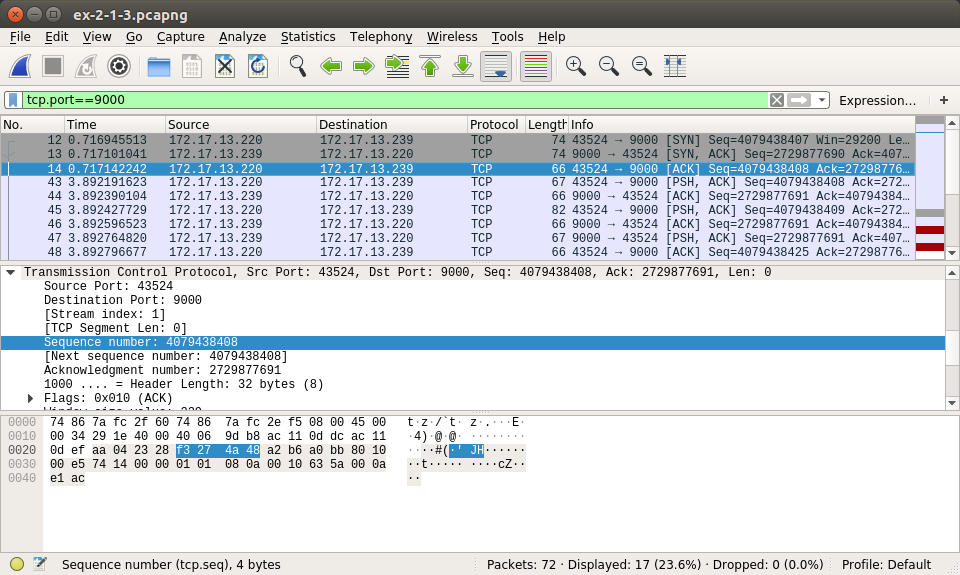
\includegraphics[width=\linewidth]{ex-2-1-4.png}
          \captionof{figure}{Número de sequência real.}
          \vspace{1em}

          O \emph{handshake} de três vias é necessário para que mesmo que haja 
          duplicatas possa-se estabelecer de forma inequivoca a conexão.
          Os números de sequẽncia vão aumentando de acordo com o procedimento.
          O \emph{host} de destino e de origem estabelecem independentemente os
          números de sequência visto que estes são obtidos através do relógio.
          Extrai-se do relógio este número de sequência e quando se responde
          no outro sentido incrementa-se um.
        \end{solution}

        \pagebreak
        \subpart
        É possível achar no campo de dados as mensagens enviadas pelo
        cliente e servidor?

        \begin{solution}
          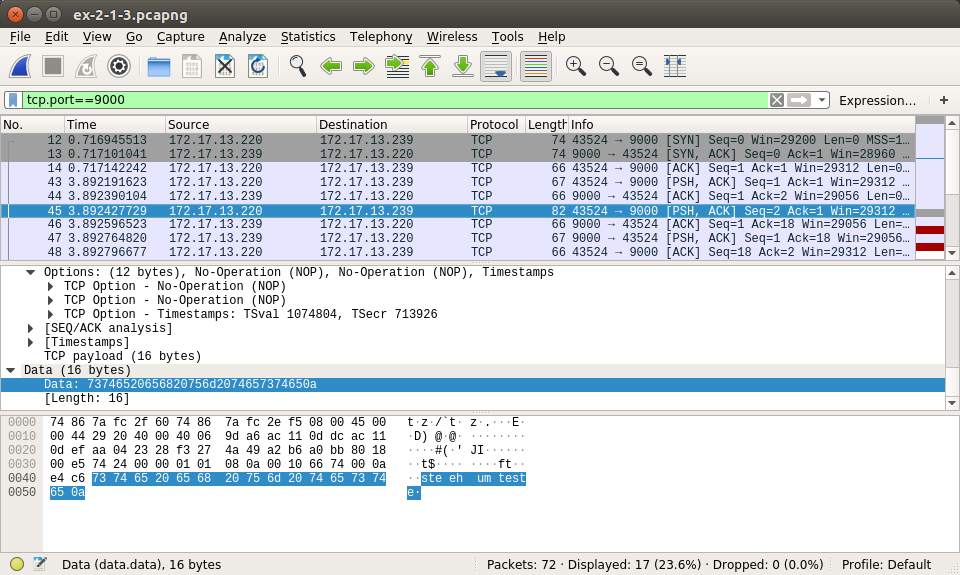
\includegraphics[width=\linewidth]{ex-2-1-5.png}
          \captionof{figure}{Um fragmento da mensagem enviada.}
          \vspace{1em}

          Sim, é possível achar no campo de dados as mensagens enviadas, onde
          estas são fragmentadas em segmentos pelo protocolo TCP.
        \end{solution}
      \end{subparts}

      \part
      Acesse a página do \href{http://www.pudim.com.br/}{Pudim}. O processo
      de estabelecimento de conexão é similar a aplicação Java?

      \begin{solution}
        Sim, o processo de estabelecimento de conexão é similar, também há
        um \emph{handshake} de três vias através do SYN, SYNACK e ACK.
      \end{solution}

      \part
      Identifique os segmentos TCP trocados entre o \emph{browser} e o Pudim,
      anotando o \href{https://tools.ietf.org/html/rfc6298}{RTT}
      (\emph{round trip time}) dos 6 primeiros segmentos.

      \begin{solution}
        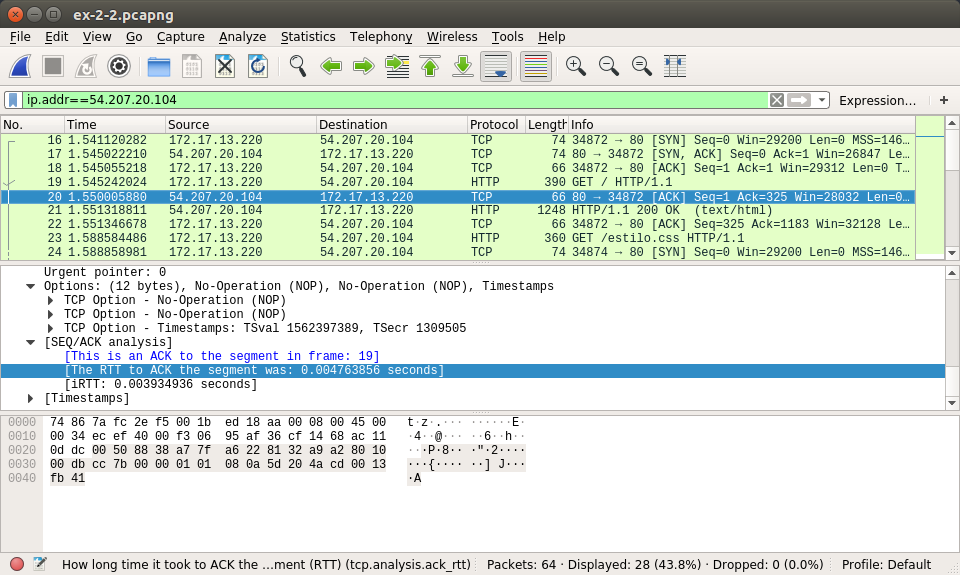
\includegraphics[width=\linewidth]{ex-2-3.png}
        \captionof{figure}{Um dos RTTs dos segmentos.}
        \vspace{1em}
        
        Diferentemente da camada de dados, é necessário sempre calcular
        o atraso para no fim obter um possível \emph{timeout}. A cada segmento
        respondido, o TCP recalcula o atraso de ida e volta.

      \begin{Verbatim}
        [The RTT to ACK the segment was: 0.003901928 seconds]
        [The RTT to ACK the segment was: 0.003901928 seconds]
        [The RTT to ACK the segment was: 0.004763856 seconds]
        [The RTT to ACK the segment was: 0.004763856 seconds]
        [The RTT to ACK the segment was: 0.004122106 seconds]
        [The RTT to ACK the segment was: 0.000031876 seconds]
      \end{Verbatim}
      \end{solution}
    \end{parts}

    \question
    Comando \verb|netstat|.

    \begin{parts}
      \part
      Execute o comando \verb|netstat -a| e comente o que se pode observar
      na saída do comando.

      \begin{solution}
        Pode-se observar os soquetes abertos e as conexões na máquina.

      \begin{Verbatim}[label={{\normalsize \$ netstat -a}}, fontsize=\scriptsize]
        Conexões Internet Ativas (servidores e estabelecidas)
        Proto Recv-Q Send-Q Endereço Local          Endereço Remoto         Estado      
        tcp        0      0 ufabc-OptiPlex-9:domain *:*                     OUÇA      
        tcp        0      0 localhost:ipp           *:*                     OUÇA      
        tcp        0      0 localhost:5893          *:*                     OUÇA      
        tcp        0      0 172.17.13.220:39666     ec2-54-218-80-178:https ESTABELECIDA
        tcp6       0      0 ip6-localhost:ipp       [::]:*                  OUÇA      
        udp        0      0 *:ipp                   *:*                                
        udp        0      0 *:mdns                  *:*                                
        udp        0      0 *:51400                 *:*                                
        udp        0      0 *:48956                 *:*                                
        udp        0      0 ufabc-OptiPlex-9:domain *:*                                
        udp        0      0 *:bootpc                *:*                                
        udp6       0      0 [::]:45436              [::]:*                             
        udp6       0      0 [::]:mdns               [::]:*                             
        raw6       0      0 [::]:ipv6-icmp          [::]:*                  7          
        Domain sockets UNIX ativos (servidores e estabelecidas)
        Proto RefCnt Flags       Type       State         I-Node   Caminho
        unix  3      [ ]         DGRAM                    765      /run/systemd/notify
        unix  2      [ ]         DGRAM                    19093    /run/user/1000/systemd/notify
        unix  2      [ ACC ]     STREAM     OUVINDO       19094    /run/user/1000/systemd/private
        [...]
      \end{Verbatim}
      \end{solution}

      \part
      Execute o comando \verb|netstat -s| e comente o que se pode observar
      na saída do comando.

      \begin{solution}
        Pode-se observar as estatísticas gerais dos protocolos.

      \begin{Verbatim}[label={\$netstat -s}]
        Ip:
            88941 total packets received
            39 with invalid addresses
            0 forwarded
            0 incoming packets discarded
            88855 incoming packets delivered
            74822 requests sent out
            44 outgoing packets dropped
        Icmp:
            112 ICMP messages received
            1 input ICMP message failed.
            Histograma de entrada ICMP:
                destination unreachable: 110
                echo requests: 2
            109 ICMP messages sent
            0 ICMP messages failed
            Histograma de saída ICMP
                destination unreachable: 107
                echo replies: 2
        [...]
      \end{Verbatim}
      \end{solution}
    \end{parts}

    \question
    Comando \verb|nmap|.

    \begin{parts}
      \part
      Execute o comando \verb|nmap -v IP|, em que \verb|IP| é o endereço IP
      da máquina a ser testada, capturando os pacotes no Wireshark. Explique
      o funcionamento do \verb|nmap|.

      \begin{solution}
        O \verb|nmap| utiliza pacotes IP para obter os \emph{hosts} disponíveis
        na rede, permitindo com que se obtenha os serviços que este está 
        executando, bem como possíveis filtros existentes no \emph{host}
        que está sendo analisado.
        
      \begin{Verbatim}[label={\$ nmap -v prograd.ufabc.edu.br}]
        Starting Nmap 7.01 ( https://nmap.org ) at 2019-04-23 11:34 -03
        Initiating Ping Scan at 11:34
        Scanning prograd.ufabc.edu.br (177.104.50.63) [2 ports]
        Completed Ping Scan at 11:34, 0.00s elapsed (1 total hosts)
        Initiating Parallel DNS resolution of 1 host. at 11:34
        Completed Parallel DNS resolution of 1 host. at 11:34, 0.00s elapsed
        Initiating Connect Scan at 11:34
        Scanning prograd.ufabc.edu.br (177.104.50.63) [1000 ports]
        Discovered open port 443/tcp on 177.104.50.63
        Discovered open port 80/tcp on 177.104.50.63
        Discovered open port 22/tcp on 177.104.50.63
        Completed Connect Scan at 11:34, 4.61s elapsed (1000 total ports)
        Nmap scan report for prograd.ufabc.edu.br (177.104.50.63)
        Host is up (0.00073s latency).
        Not shown: 996 filtered ports
        PORT     STATE  SERVICE
        22/tcp   open   ssh
        80/tcp   open   http
        443/tcp  open   https
        8080/tcp closed http-proxy
        
        Read data files from: /usr/bin/../share/nmap
        Nmap done: 1 IP address (1 host up) scanned in 4.66 seconds
      \end{Verbatim}
      \end{solution}
    \end{parts}
  \end{questions}
\end{document}
